\documentclass[14pt]{beamer}

% Presento style file
\usepackage{config/presento}
% custom command and packages
\input{config/custom-command}
% My macros
/Users/zach/Git/zachs_macros/zachs_macros.tex

% Custom colors
\usepackage{color}
\definecolor{ao}{rgb}{0.0, 0.5, 0.0}

% Configure listings for R
\usepackage{listings}

\lstset{frame=tb,
language=R,
keywordstyle=\color{blue},
otherkeywords={!,!=,~,$,*,\&,\%/\%,\%*\%,\%\%,<-,<<-,\%>\%},
alsoletter={.,_}
}

% Information
\title{LOST IN HYPERSPACE}
\subtitle{\emph{The Curse of Dimensionality}}
\author{Zachary del Rosario}
\institute{zdr@stanford.edu}
\date{September 6th}
%% \date{\today}

% For latex 2018
\makeatletter
\let\@@magyar@captionfix\relax
\makeatother

% --------------------------------------------------
\begin{document}
% --------------------------------------------------

% --------------------------------------------------
\framecard[colorgreen]{{\color{white}\hugetext{%
      \centering%
      Please print your\\
      name on a card!
}}}

% -------------------------
\begin{frame}[plain]
\maketitle
\end{frame}

% --------------------------------------------------
%% SEC: My Background
% --------------------------------------------------
\framepicv[1.0]{images/olin_compressed}{} % Olin

% -------------------------
\framepicv[1.0]{images/seq}{} % Stanford Engineering Quad

% -------------------------
\framecard[colorgreen]{{\color{white}\hugetext{%
      \centering%
      ICME
}}}

% --------------------------------------------------
%% SEC: Planes -> Dimensionality
% --------------------------------------------------
\framepicv[1.0]{images/lax_shuttle-25p}{
 \begin{textblock}{7}(0.0,5.7)
    {\tiny By Aaron Barnaby aaronbarnaby}
 \end{textblock}
}

% -------------------------
\framepicv[0.8]{images/gipsy_moth-25p}{
 \begin{textblock}{7}(0.0,5.7)
    {\tiny By Peripitus - Own work, CC BY-SA 3.0}
 \end{textblock}%
 \textblockcolor{white}
 \textblockrulecolor{black}
 \only<2>{
   \begin{textblock}{4.5}(0.0,3.5)
     {
       \begin{tabular}{l|l}
       \hline
       Strength & Spar1\\
       \hline
       Stress? & Size?\\
       \hline
       \end{tabular}
     }
   \end{textblock}
 }%
 \only<3>{
   \begin{textblock}{6.2}(0.0,3.5)
     {
       \begin{tabular}{l|l|l}
       \hline
       Strength & Spar1 & Spar2\\
       \hline
       Stress? & Size? & Size?\\
       \hline
       \end{tabular}
     }
   \end{textblock}
 }%
 \only<4>{
   \begin{textblock}{11.0}(0.0,3.5)
     {
       \begin{tabular}{l|l|l|l|l|l}
       \hline
       Strength & Spar1 & Spar2 & Rib1 & Rib2 & Rib3\\
       \hline
       Stress? & Size? & Size? & Size? & Size? & Size?\\
       \hline
       \end{tabular}
     }
   \end{textblock}
 }%
 \textblockcolor{}
 \textblockrulecolor{}
}

% -------------------------
\begin{frame}[plain]
 \textblockcolor{}
 \textblockrulecolor{}
  \only<1>{%
    \begin{textblock}{11}(-0.5,-1.5)
      {\textblockcolour{}
        \small
        \begin{tabular}{l|r}
        \hline
        Str & Spar1\\
        \hline
        ? & 1\\
        \hline
        ? & 2\\
        \hline
        ? & 3\\
        \hline
        \end{tabular}
      }
    \end{textblock}
    \begin{tikzpicture}[remember picture,overlay]
      \node[xshift=+3cm,yshift=+1.5cm] at (current page.center){%
        \includegraphics[width=6cm]{./images/points1}};
    \end{tikzpicture}
  }
  \only<2>{%
    \begin{textblock}{11}(-0.5,-1.5)
      {\textblockcolour{}
        \small
        \begin{tabular}{l|r|r}
        \hline
        Str & Spar1 & Spar2\\
        \hline
        ? & 1 & 1\\
        \hline
        ? & 2 & 1\\
        \hline
        ? & 3 & 1\\
        \hline
        ? & 1 & 2\\
        \hline
        ? & 2 & 2\\
        \hline
        ? & 3 & 2\\
        \hline
        ? & 1 & 3\\
        \hline
        ? & 2 & 3\\
        \hline
        ? & 3 & 3\\
        \hline
        \end{tabular}
      }
    \end{textblock}
    \begin{tikzpicture}[remember picture,overlay]
      \node[xshift=+3cm,yshift=+1.5cm] at (current page.center){%
        \includegraphics[width=6cm]{./images/points2}};
    \end{tikzpicture}
  }
  \only<3->{%
    \begin{textblock}{11}(-0.5,-1.5)
      {\textblockcolour{}
        \small
        \begin{tabular}{l|r|r|r}
        \hline
        Str & Spar1 & Spar2 & Rib1\\
        \hline
        ? & 1 & 1 & 1\\
        \hline
        ? & 2 & 1 & 1\\
        \hline
        ? & 3 & 1 & 1\\
        \hline
        ? & 1 & 2 & 1\\
        \hline
        ? & 2 & 2 & 1\\
        \hline
        ? & 3 & 2 & 1\\
        \hline
        ? & 1 & 3 & 1\\
        \hline
        ? & 2 & 3 & 1\\
        \hline
        ? & 3 & 3 & 1\\
        \hline
        \vdots & \vdots & \vdots & \vdots
        \end{tabular}
      }
    \end{textblock}
    \begin{tikzpicture}[remember picture,overlay]
      \node[xshift=+3cm,yshift=+1.5cm] at (current page.center){%
        \includegraphics[width=6cm]{./images/points3}};
    \end{tikzpicture}
  }
  % Annotation
  \only<4->{
    \begin{textblock}{5}(5.5,2.5)
      {\textblockcolor{}
        That's a lot of planes! \\
        \only<5>{%
          \alert{Make a prediction:} How many planes for $d$ variables?\\
          Maybe $\approx d$? $\approx d^2$?
        }
      }
    \end{textblock}
  }
\end{frame}

% -------------------------
\framepich[0.8]{images/full_747}{
 \begin{textblock}{7}(0.0,5.7)
    {\tiny Jameson et al. (1986)}
 \end{textblock}
}

% -------------------------
\framepich[0.7]{images/titan_render}{
  \only<2>{
    \begin{textblock}{7}(0.0,4.5)
      {Simulations run\\ hours to \emph{months}}
    \end{textblock}
  }
}

% -------------------------
\begin{frame}[t]{Thought Experiment}
  Suppose our simulation ran in \emph{one second}, \\
  and we use $10$ points per dimension....

  \bigskip
  \only<2->{How long would this take to execute?\\}
  \only<3>{%
    Scaling is \emph{exponential}, i.e.
    \begin{equation*}
      \text{Time} = C^d
    \end{equation*}
  }
\end{frame}

% -------------------------
\framepicv[0.8]{images/dimensionality}{
  \only<2>{%
    \begin{textblock}{7}(3.8,3.0)
        {\textblockcolor{}
          \alert{The Curse of Dimensionality}
        }
    \end{textblock}
  }
}

% --------------------------------------------------
%% SEC: Outline
% --------------------------------------------------
\begin{frame}{Outline}
  \begin{itemize}
  \item 1. \emph{Accursed} Data
  \item 2. \emph{Accursed} Geometry
  \item 3. Lifting the Curse...
  \item 4. An Activity
  \end{itemize}
\end{frame}

% --------------------------------------------------
%% SEC: Big Data
% --------------------------------------------------
\framecard[colorgreen]{{\color{white}\hugetext{%
      \centering%
      Big Data\\
      and\\
      Dimensionality
}}}

% -------------------------
\begin{frame}{The Data Matrix}
  We've already seen one of these!

  \begin{table}
    \begin{tabular}{l|r|r|r}
      \hline
      Str & Spar1 & Spar2 & Rib1\\
      \hline
      ? & 1 & 1 & 1\\
      \hline
      ? & 2 & 1 & 1\\
      \hline
      ? & 3 & 1 & 1\\
      \hline
      ? & 1 & 2 & 1\\
      \hline
      ? & 2 & 2 & 1\\
      \hline
      ? & 3 & 2 & 1\\
      \hline
      ? & 1 & 3 & 1\\
      \hline
      ? & 2 & 3 & 1\\
      \hline
      ? & 3 & 3 & 1\\
      \hline
      \vdots & \vdots & \vdots & \vdots
    \end{tabular}
  \end{table}
\end{frame}

% -------------------------
\begin{frame}{The Data Matrix}
  % Content
  \begin{table}
    \begin{tabular}{@{}l|l|l|l@{}}
                      & Variable $1$ & $\cdots$ & Variable $d$ \\
      \hline
      Observation $1$ & $42$         & $\vdots$ & $0451$ \\
      $\vdots$        & $\vdots$     & $\vdots$ & $\vdots$
    \end{tabular}
  \end{table}
  % Annotation
  \only<2->{%
    \begin{textblock}{7}(4.0,-4.0)
      {\textblockcolor{}
        Every \alert{column} is a \alert{variable}\\
        \only<4->{Increasing dimensionality $\rhd$}
      }
    \end{textblock}
  }
  \only<3->{%
    \begin{textblock}{7}(+0.5,+1.0)
      {\textblockcolor{}
        Every \alert{row} is an \alert{observation}\\
        \only<4->{Increasing observations $\bigtriangledown$}
      }
    \end{textblock}
  }
  \only<5>{%
    \begin{textblock}{12}(-0.5,+0.0)
      {\textblockcolor{}
        \LARGE Both contribute to `Big Data'
      }
    \end{textblock}
  }
\end{frame}

% -------------------------
\framecard[colorblue]{{\color{white}%

``The trend today is towards more observations \emph{but even more so},
    \alert{to radically larger numbers of variables} – voracious, automatic,
    systematic collection of hyper-informative detail about each observed
    instance.''

    \bigskip
    -- David Donoho, 2000\\
    \tiny (Emphasis added)

}}

% -------------------------
\begin{frame}{How Big is our Data?}
  \begin{itemize}
  \item<1-> How many entries in a data matrix?\\
    \visible<2->{\alert<2>{%
      -- Observations $\times$ Dimensionality
    }}

    \bigskip
  \item<3-> How many Observations needed for Dimensionality?\\
    \visible<4->{\alert<4>{%
      -- Exponential in Dimensionality\textsuperscript{*}
    }}

    \bigskip
  \item<5-> How many hard drives will we need?!

    \bigskip
  \item<6> What's so special about high dimensionality?
  \end{itemize}
\end{frame}

% --------------------------------------------------
%% SEC: High-dimensional geometry
% --------------------------------------------------
\framecard[colorgreen]{{\color{white}\hugetext{%
      \centering%
      Weird Facts\\
      about\\
      High-\\
      Dimensional\\
      Geometry
}}}

% -------------------------
\begin{frame}{Fact 1}
  Basic solids defy intuition
\end{frame}

% -------------------------
\begin{frame}{Sketching Solids}
  Hyperspheres and Hypercubes
\end{frame}

% -------------------------
\begin{frame}[plain]
  \begin{textblock}{7}(-0.5,-3.5)
    {\textblockcolor{}
      Hypercube on $[-\f12,+\f12]^d$\\
      Hypersphere of radius $1$\\
      Which is bigger for $d = 2$?
    }
  \end{textblock}
\end{frame}

% -------------------------
\framepich[1.0]{images/box_in_sphere1}{
  % Annotation
  \begin{textblock}{2}(+0.5,+4.0)
    {\textblockcolor{}
      $d = 2$
    }
  \end{textblock}

  % Footer
  \begin{textblock}{7}(0.0,5.7)
    {\tiny By Venkatesan Guruswami}
  \end{textblock}
}

% -------------------------
\framepich[1.0]{images/box_in_sphere2}{
  % Annotation
  \begin{textblock}{2}(+0.5,+4.0)
    {\textblockcolor{}
      $d = 2$
    }
  \end{textblock}

  \begin{textblock}{2}(+4.7,+4.0)
    {\textblockcolor{}
      $d = 4$
    }
  \end{textblock}

 \begin{textblock}{7}(0.0,5.7)
    {\tiny By Venkatesan Guruswami}
 \end{textblock}
}

% -------------------------
\framepich[1.0]{images/box_in_sphere3}{
  % Annotation
  \begin{textblock}{2}(+0.5,+4.0)
    {\textblockcolor{}
      $d = 2$
    }
  \end{textblock}

  \begin{textblock}{2}(+4.7,+4.0)
    {\textblockcolor{}
      $d = 4$
    }
  \end{textblock}

  \begin{textblock}{2}(+9.0,+4.0)
    {\textblockcolor{}
      $d \to \infty$
    }
  \end{textblock}

 \begin{textblock}{7}(0.0,5.7)
    {\tiny By Venkatesan Guruswami}
 \end{textblock}
}

% -------------------------
\begin{frame}{Fact 2}
  The hypersphere has vanishing interior
\end{frame}

% -------------------------
\begin{frame}{Unit Hypersphere Volume}
  \begin{equation*} \begin{aligned}
      HV &= \frac{\pi ^ {d / 2}}{\Gamma(d / 2 + 1)}\\
      \visible<2>{%
        &= \int\cdots\int \alert{r^{d-1}}\,
           T(\varphi_{1},\dots,\varphi_{d-1})\,
           dr d\varphi_{1}\cdots d\varphi_{d-1}
      }
  \end{aligned} \end{equation*}
\end{frame}

% -------------------------
\framepicv[0.8]{images/surface_density}{}

% -------------------------
\begin{frame}{Fact 3}
  Johnson-Lindenstrauss Lemma....
\end{frame}

% -------------------------
\begin{frame}{We Will Study:}
  \underline{Claim}: For any $0<\epsilon<1$ and $n\in\mathbb{Z}_{>0}$, let
  $k\in\mathbb{Z}_{>0}$ such that

  \begin{equation*}
    k \geq C \frac{\log(n)}{\epsilon^2},
  \end{equation*}

  \noindent then for all sets of points $V\subset\R{d}$, there is a projection
  $P_k:\R{d}\to\R{k}$ such that, for all $u,v\in V$, we have

    \begin{equation*}
      \alert<2>{(1 - \epsilon)\|\vu - \vv\|^2 \leq \|P_k(\vu) - P_k(\vv)\|^2 \leq %
      (1 + \epsilon)\|\vu - \vv\|^2
}    \end{equation*}
\end{frame}

% JL: Distance
% -------------------------
\begin{frame}{}
  % Content
  \only<-5>{%
    \begin{equation*} \begin{aligned}
        (1 - \alert<3>{\epsilon})(\alert<2>{\text{Distance}})^2 &\leq %
          (\alert<4,5>{\text{Projected Distance}})^2 \\
        &\, \\
        (\alert<4,5>{\text{Projected Distance}})^2 &\leq %
          (1 + \alert<3>{\epsilon})(\alert<2>{\text{Distance}})^2\\
    \end{aligned} \end{equation*}
  }%
  % Annotation
  \visible<2-5>{%
    \begin{textblock}{3}(+1.5,-5.7)
      {\textblockcolor{}
        \centering%
        \only<2>{\includegraphics[width=1.0\textwidth]{./images/proj0_alert}}
        \only<3-5>{\includegraphics[width=1.0\textwidth]{./images/proj0}}
      }
    \end{textblock}
  }
  \visible<3-5>{%
    \begin{textblock}{3}(+5.5,-4.0)
      {\textblockcolor{}
        \alert<3>{$\epsilon$ is \emph{small}}
      }
    \end{textblock}
  }
  \visible<4-5>{%
    \begin{textblock}{3}(-0.5,+0.0)
      {\textblockcolor{}
        \centering%
        \only<4>{\includegraphics[width=1.0\textwidth]{./images/proj1_alert}}
        \only<5>{\includegraphics[width=1.0\textwidth]{./images/proj1}}
      }
    \end{textblock}
  }
  \visible<5-5>{%
    \begin{textblock}{3}(+3.0,+0.0)
      {\textblockcolor{}
        \centering\includegraphics[width=1.0\textwidth]{./images/proj2_alert}
      }
    \end{textblock}
  }
\end{frame}

% JL: Projections
% -------------------------
\begin{frame}[t]{}
  % Content
  \begin{equation*}
    (1 - \epsilon)\|\vu - \vv\|^2 \leq \|P_{\alert{k}}(\vu) - P_{\alert{k}}(\vv)\|^2 \leq %
    (1 + \epsilon)\|\vu - \vv\|^2
  \end{equation*}
  % Annotation
  \visible<2->{%
    \begin{textblock}{6}(+2.5,-0.5)
      {\textblockcolor{}
        \centering%
        \only<2>{\includegraphics[width=1.0\textwidth]{./images/dim_proj3}}
        \only<3>{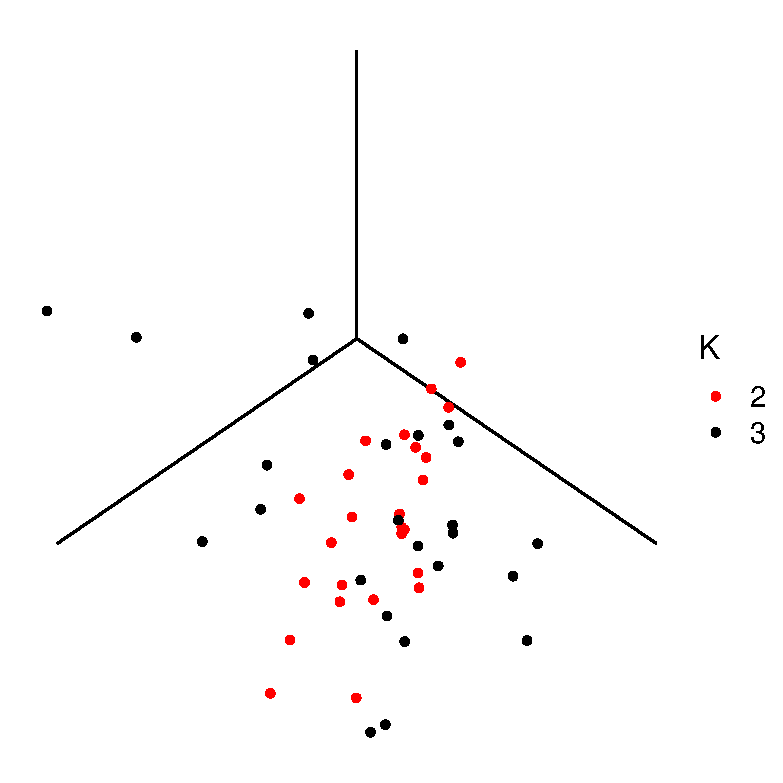
\includegraphics[width=1.0\textwidth]{./images/dim_proj2}}
        \only<4>{\includegraphics[width=1.0\textwidth]{./images/dim_proj1}}
      }
    \end{textblock}
  }
\end{frame}

% JL: Dimensionality
% -------------------------
\begin{frame}{}
  % Content
  \begin{equation*}
    \alert<2>{k} \geq C\frac{\log(\alert<3>{n})}{\alert<4>{\epsilon}^2}
  \end{equation*}
  % Annotation
  \visible<2->{%
    \begin{textblock}{4}(+0.0,-3.5)
      {\textblockcolor{}
        $k$ is the projection dimension
      }
    \end{textblock}
  }
  \visible<3->{%
    \begin{textblock}{4}(+0.0,+2.0)
      {\textblockcolor{}
        $n$ is the number of observations
      }
    \end{textblock}
  }
  \visible<4->{%
    \begin{textblock}{4}(+7.0,+2.0)
      {\textblockcolor{}
        $\epsilon$ is the desired error
      }
    \end{textblock}
  }
  \visible<5->{%
    \begin{textblock}{4.5}(+7.0,-3.5)
      {\textblockcolor{}
        Dimensionality is\\
        \emph{curiously absent!}
      }
    \end{textblock}
  }
\end{frame}

% JL: Example
% -------------------------
\begin{frame}[fragile]{JL: Example}
Example: Gene expression levels for tumor types BRCA, KIRC, COAD, LUAD and PRAD.

\bigskip
  \begin{lstlisting}
## Gene data from UCI
dim(gene_data)
#       Obs,  Dim
> [1]   801 20531
  \end{lstlisting}

  \bigskip
  Note: This code on GitHub: https://github.com/zdelrosario/hyperspace
\end{frame}

% -------------------------
\begin{frame}[fragile]{JL: Example}
  \begin{lstlisting}
C <- 2                 # Over-samping
eps <- 0.1             # 10% distort
n <- dim(gene_data)[1] # Observations
d <- dim(gene_data)[2] # Dimension

k <-  ceiling(C * log(n) / eps ^ 2)
k
> 1338 (6.5% of 20531)
  \end{lstlisting}
\end{frame}

% -------------------------
\begin{frame}[fragile]{JL: Example}
  \begin{lstlisting}
## Randomly project
P_k <- random_projection(k x d)
projected_data = gene_data %*% P_k
  \end{lstlisting}
\end{frame}

% -------------------------
\begin{frame}[fragile]{JL: Example}
  \begin{lstlisting}
eps
# Requested distortion
>    10%
quantile(relative_difference)
# Quantile
>      0%     25%    50%    75%   100%
# Realized distortion
> -7.784% -1.193% 0.082% 1.344% 8.139%
  \end{lstlisting}
\end{frame}

% --------------------------------------------------
%% SEC: Dimension Reduction
% --------------------------------------------------
\framecard[colorgreen]{{\color{white}\hugetext{%
      \centering%
      Lifting\\
      the\\
      Curse
}}}

% -------------------------
\begin{frame}{Dimension Reduction}
  \huge\underline{Idea:} Find \emph{low-dimensional} structure in data
\end{frame}

% -------------------------
\begin{frame}{Ex: Low-Dimensional Structure}
  Example: FAA Aircraft characteristic database

  \bigskip
  \begin{tabular}{@{}ll@{}}
    Variable & Description \\
    \hline
    wingspan    & Wingspan [ft] \\
    length      & Length [ft] \\
    tail\_height & Tail height [ft] \\
    cmg         & Cockpit-to-main gear [ft] \\
    mgw         & Main gear width [ft] \\
    mtow        & Maximum take-off weight [lbs] \\
    approach\_speed & Approach speed [kts]
  \end{tabular}
\end{frame}

% -------------------------
\begin{frame}{Ex: Low-Dimensional Structure}
  \begin{figure}
    \centering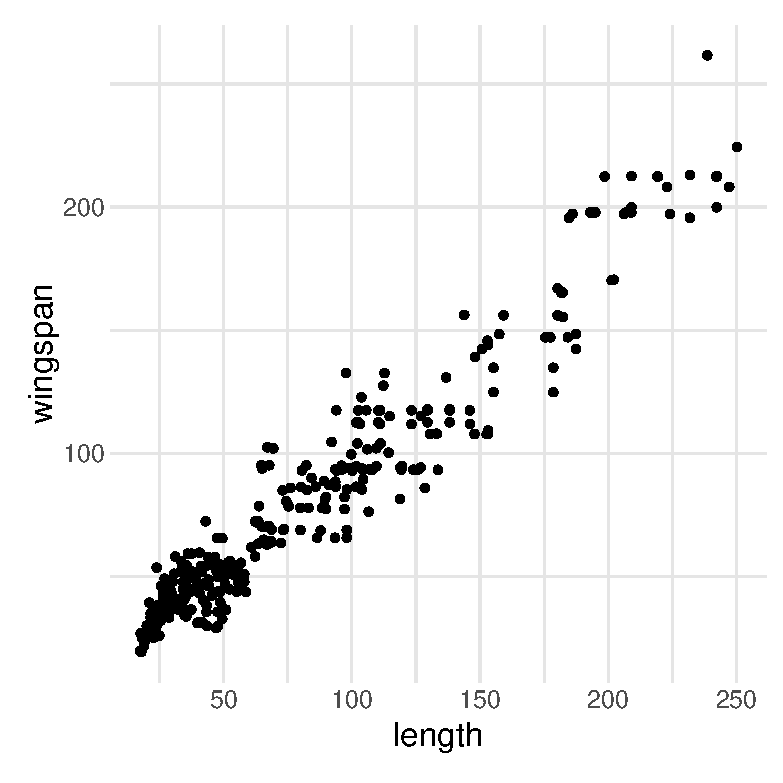
\includegraphics[width=0.7\textwidth]{./images/faa_wingspan_v_length}
  \end{figure}
\end{frame}

% -------------------------
\begin{frame}{Ex: Low-Dimensional Structure}
  \begin{figure}
    \centering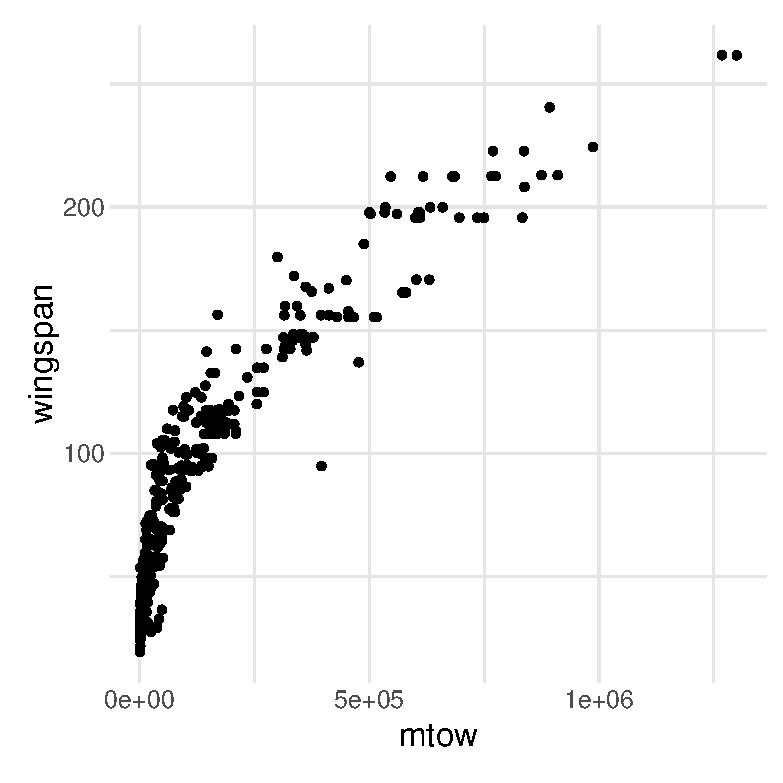
\includegraphics[width=0.7\textwidth]{./images/faa_wingspan_v_mtow}
  \end{figure}
\end{frame}

% -------------------------
\begin{frame}{Ex: Low-Dimensional Structure}
  \begin{figure}
    \centering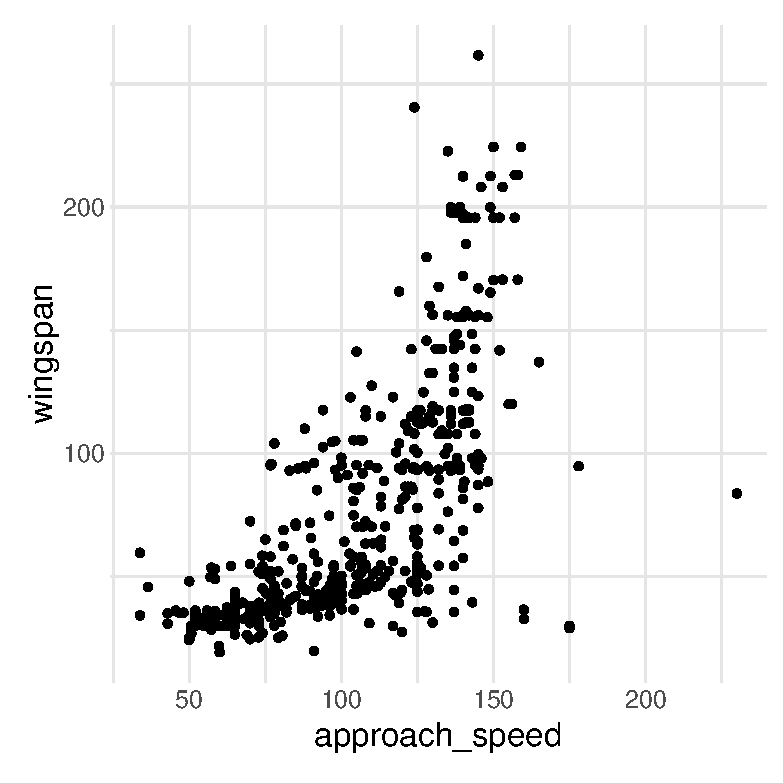
\includegraphics[width=0.7\textwidth]{./images/faa_wingspan_v_approach_speed}
  \end{figure}
\end{frame}

% -------------------------
\begin{frame}{Ex: Scatterplot Matrix}
  \begin{figure}
    \centering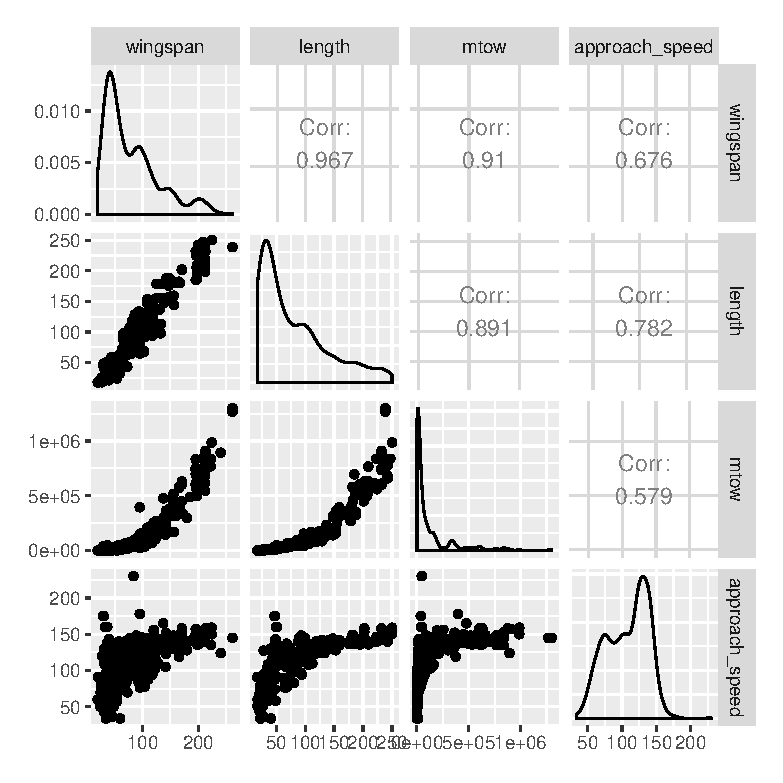
\includegraphics[width=0.7\textwidth]{./images/faa_min_scatter}
  \end{figure}
\end{frame}

% -------------------------
\begin{frame}{Ex: Scatterplot Matrix, log}
  \begin{figure}
    \centering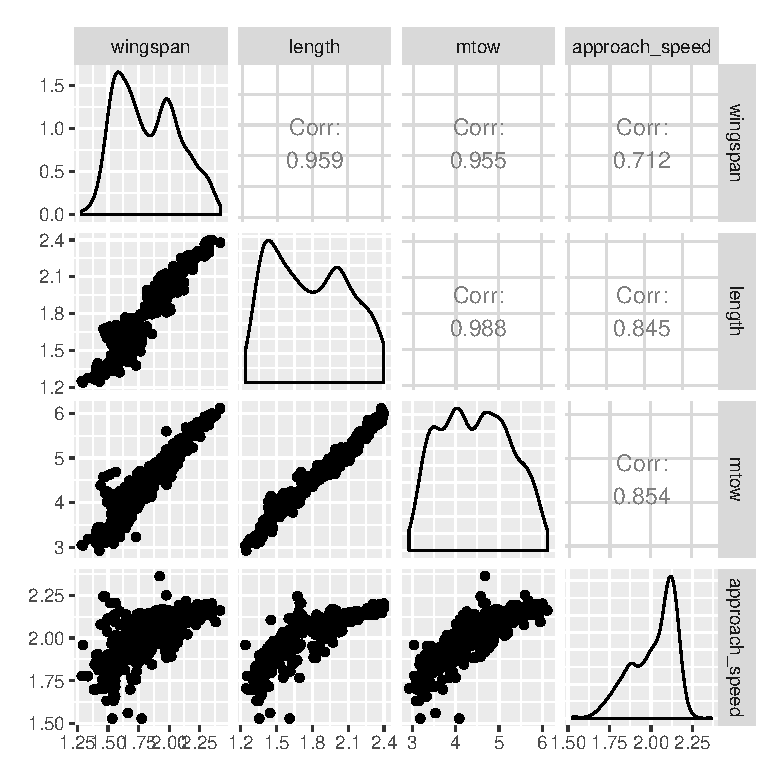
\includegraphics[width=0.7\textwidth]{./images/faa_min_scatter_log}
  \end{figure}
\end{frame}

% -------------------------
\begin{frame}{Methods}
  \begin{itemize}
  \item Random projections -- JL
  \item Important directions -- PCA
  \end{itemize}
\end{frame}

% -------------------------
\begin{frame}{Important Directions}
  \huge\underline{Idea:} Find directions that capture variability
\end{frame}

% -------------------------
\framepicv[1.0]{images/pca1}{}
\framepicv[1.0]{images/pca2}{}
\framepicv[1.0]{images/pca3}{
  \visible<2>{
    \begin{textblock}{7}(4.5,5.0)
      {\textblockcolor{}
        Direction \alert{from data}
      }
    \end{textblock}
  }
}

% -------------------------
\begin{frame}[fragile]{Ex: PCA}
  \begin{lstlisting}
df_min_pca <-
    df_faa %>%
    tidy_pca(wingspan, length, mtow, approach_speed)

df_min_pca %>%
    pull(pc_frac)
> | k |  Var  | Frac |
> |--:|------:|-----:|
> | 1 | 1.85  |  62% |
> | 2 | 0.68  |  85% |
> | 3 | 0.29  |  95% |
> | 4 | 0.15  | 100% |
  \end{lstlisting}
\end{frame}

% --------------------------------------------------
%% SEC: Activity
% --------------------------------------------------
\framecard[colorgreen]{{\color{white}\hugetext{%
      \centering%
      Activity!
}}}

\end{document}
